\section{Introduction}
\begin{figure}
\centering
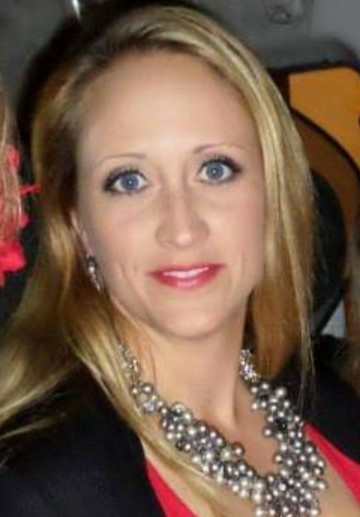
\includegraphics[scale=0.5]{putman.jpg}
\end{figure}
 \subsection{My Background}
My name is Cassandra Putman. My background has focused in mathematics and systems engineering.  Recently, I have decided to branch out into computer science and obtain a Master of Engineering in Cyber Security with an intent of focusing on hardware security.  I have a 17 year career in Department of Defense space systems including launch vehicles, space vehicles and most recently the ground systems that support the space vehicles.  System security, including software, hardware and physical security are of utmost importance to all the space programs I have worked, as they are often national security asset systems.
\subsection{My Research Interests and Course Goals}
I intend to focus my research in supply chain security with a focus on hardware security. While I'm fairly new to the computer science field and only recently started learning about blockchain, I do see a great utility and applicability being possible in applying blockchain technology to improve hardware supply chain security.  It appears, in my initial research, that applying blockchain technology to an IT supply chain, especially a supply chain that is as controlled as those that exist in government contracting, is both feasible and capable of providing great security benefits to the system, the user, and ultimately the security of the nation. I hope to narrow my research topic during this course and develop a focused and novel idea in the area of hardware supply chain security.
\subsection{My Personal Interests}
While I enjoy math and often read math related books, I also love to volunteer with a shar pei rescue.  I volunteer by performing temperament evaluations, transporting and fostering dogs and  performing home checks for potential fosters and adopters.  I have fostered 100+ dogs in the 12 years I have been volunteering with the shar pei rescue.  Beyond dog rescue, I also enjoy reading, hiking and doing crafts such as sewing and kitting. My love for travel has taken me to over 20 countries in the world, and I have plans to hit many more.  Figure 1 is a picture of me.

\textbf{Question from Maria Psarakis to Cassandra Putman:} I'm so impressed with your DoD background, did it have you living in lots of different places in the world? I'm equally impressed with everyone who quilts, sews, knits...how did you get started knitting? 
<<<<<<< HEAD

\textbf{Answer to Maria:} When I first joined the Air Force I had big dreams of seeing the country and going overseas, travelling the world.  Instead, I lived in a cubicle in Los Angeles Air Force Base. I was lucky that I had amazing jobs, because LA was not what I had in mind.  But satellites and especially launch vehicle work made it worth it!  Since I didn't get to do any serious travel with the military, I made a goal to go somewhere international at least once each year.  Until this year (thanks to COVID), I've kept that goal and I've been to ~20 countries (Republic of Georgia on the top of that list if you ever get a chance!) 
=======
Maria: When I first joined the Air Force I had big dreams of seeing the country and going overseas, travelling the world.  Instead, I lived in a cubicle in Los Angeles Air Force Base. I was lucky that I had amazing jobs, because LA was not what I had in mind.  But satellites and especially launch vehicle work made it worth it!  Since I didn't get to do any serious travel with the military, I made a goal to go somewhere international at least once each year.  Until this year (thanks to COVID), I've kept that goal and I've been to ~20 countries (Republic of Georgia on the top of that list if you ever get a chance!) 
>>>>>>> 395e345b13e2f4e534ee67e0916c1dac96bbad64
As far as knitting (and sewing) go, I got started in high school. My best friend's gramdmother taught her and she taught me. I still have the first blanket I knitted, in the heat of summer between my junior and senior year of high school. Imagine being that cool! 
